\documentclass[eng,printmode,oneside]{mgr}
%opcje klasy dokumentu mgr.cls zostaly opisane w dolaczonej instrukcji

%ponizej deklaracje uzycia pakietow, usunac to co jest niepotrzebne
\usepackage{polski} %przydatne podczas skladania dokumentow w j. polskim
%\usepackage[polish]{babel}%alternatywnie do pakietu polski, wybrac jeden z nich
\usepackage[utf8]{inputenc} %kodowanie znakow, zalezne od systemu
\usepackage[T1]{fontenc} %poprawne skladanie polskich czcionek
\usepackage{wrapfig}

%listingi
\usepackage{listings}
\usepackage{color}
\definecolor{zielony}{rgb}{0,0.6,0}
\definecolor{innyZielony}{rgb}{0.5,0.7,0}
\renewcommand{\lstlistingname}{Listing}% Listing -> Algorithm
\renewcommand{\lstlistlistingname}{List of \lstlistingname s}% 
\usepackage[justification=centering]{caption}
\usepackage[pdftex]{graphicx}
\usepackage{sidecap}

%kolor do komentarzy, uwag, przypomnienie
\definecolor{komentarz}{rgb}{1,0,0}

%pakiety do grafiki
\usepackage{graphicx}
\usepackage{subfigure}
\usepackage{psfrag}

%pakiety dodajace duzo dodatkowych polecen matematycznych
\usepackage{amsmath}
\usepackage{amsfonts}

%pakiety wspomagajace i poprawiajace skladanie tabel
\usepackage{supertabular}
\usepackage{array}
\usepackage{tabularx}
\usepackage{hhline}

%pakiet wypisujacy na marginesie etykiety rownan i rysunkow zdefiniowanych przez \label{}, chcac wygenerowac finalna wersje dokumentu wystarczy usunac 
%ponizsza linie
\usepackage{showlabels}

%definicje wlasnych polecen
\newcommand{\R}{I\!\!R} %symbol liczb rzeczywistych, dziala tylko w trybie matematycznym
\newtheorem{theorem}{Twierdzenie}[section] %nowe otoczenie do skladania twierdzen

%dane do zlozenia strony tytulowej
\title{System monitoringu lokalizacji przesyłek kurierskich}
\engtitle{English title ŁŁĄŚŹĆŻÓ łąśćźżóę Ę}
\author{Monika Strachowska}
\supervisor{dr hab. inz. Imie Nazwisko Prof. PWr, I-6}
%\guardian{dr hab. inz. Imie Nazwisko Prof. PWr, I-6} %nie uzywac jesli opiekun jest ta sama osoba co prowadzacy prace

%\date{2008} %standardowo u dolu strony tytulowej umieszczany jest biezacy rok, to polecenie pozwala wstawic dowolny rok

%ponizej jest lista kierunkow i specjalnosci na wydziale elektroniki, nalezy wybrac wlasciwe lub dopisac jesli nie ma odpowiednich
\field{Automatyka i Robotyka (AIR)}
\specialisation{Systemy informatyczne w automatyce (ASI)}

%tutaj zaczyna sie wlasciwa tresc dokumentu
\begin{document}

\lstdefinestyle{listJava}{language=Java, breaklines=true,
commentstyle=\color{zielony},frame=single, numbers=left, stepnumber=1,
numbersep=5pt}
\lstdefinestyle{listPython}{language=Python, breaklines=true,
commentstyle=\color{innyZielony},frame=single, numbers=left, stepnumber=1,
numbersep=5pt}

\bibliographystyle{plabbrv} %tylko gdy uzywamy BibTeXa, ustawia polski styl bibliografii

\maketitle %polecenie generujace strone tytulowa


\tableofcontents %spis tresci

%ponizej znajduje sie przykladowa tresc dalszej czesci dokumentu, zainteresowanych zachecam do rozszyfrowania frazy "Lorem ipsum" :)
\chapter{Wstęp i cel pracy}

Współcześnie coraz więcej osób korzysta z możliwości zakupów przez internet,
niesie to za sobą wiele korzyści. Często zakupiony towar jest tańszy, unikalny,
bądz niedostępny w stacjonarnym sklepie czy poprostu jest to wygodniejsza forma
zakupów. Oprócz wyżej wymienionych zakupów istotnym towarem przewożonym
są dokumenty, często szybko potrzebne. Z tych powodów ludzie zamawijący usługi 
kurierskie chcieliby dostać jak najwyższą jakość. Zwiększenie jakości tej
usługi może nastąpić poprzez skrócenie czasu dostarczenia przesyłki(co
fizycznie już jest nie osiągalne), tańszy jej koszt, czy na przykład możliwość
sprawdzenia, w jakim dokładnie miejscu ona się znajduje. Dokładna lokalizacja
przesyłki - taka funkcjonalność usługi kurierskiej nie należy do jakości
wymaganej i koniecznej, ale znacznie podniesie prestiż firmy
kurierskiej, która zdecyduje się na taką dodatkową funkcjonalność. Z punktu
widzenia klienta odczuwany jest komfort informacji, gdzie jest przesyłka, dzięki
temu klient może zaplanować sobie dzień, w którym nastąpi dostarczenie. 

Przedstawiany tu projekt rozwija aktualną funkcjonalność firm kurierskich o
graficzne przedstawienie, w formie mapy, aktualnej lokalizacji przesyłki. Taka
forma prezentacji jest prosta w odbiorze i bardziej czytelna niż wyniki
jakie prezentowane są aktualnie w formie tabel, w których zawarte są miejsca
odbicia przesyłki. Ponadto praca próbuje rozwiązać problem jaki istnieje w
estymacji czasu dostraczaniu przesyłki do adresata, esytmacja czasu
dostarczenia jest bardzo niedokładna(ogólna) lub jej nie ma.

\emph{\color{komentarz}
Projekt został zrealizowany z wykorzystaniem takich
technologi jak:
język programowania Java, system operacyjny Android, baza danych MySQL, Google Apps.
http://www.lokalizacja.info/pl/testy/monitoring/gdzie-jest-moja-paczka-test-firm-kurierskich.html\#.VEzCPVS988o
Firmy kurierskie maja najprawdopodobniej system „windows ce/mobile” na swoich urządzenia. Ja ze względu na brak takiego urządzenia (mobilnego z windowsem) 
zrealizuje zadanie na androidzie.
}

\begin{figure}[ht!]
\centering
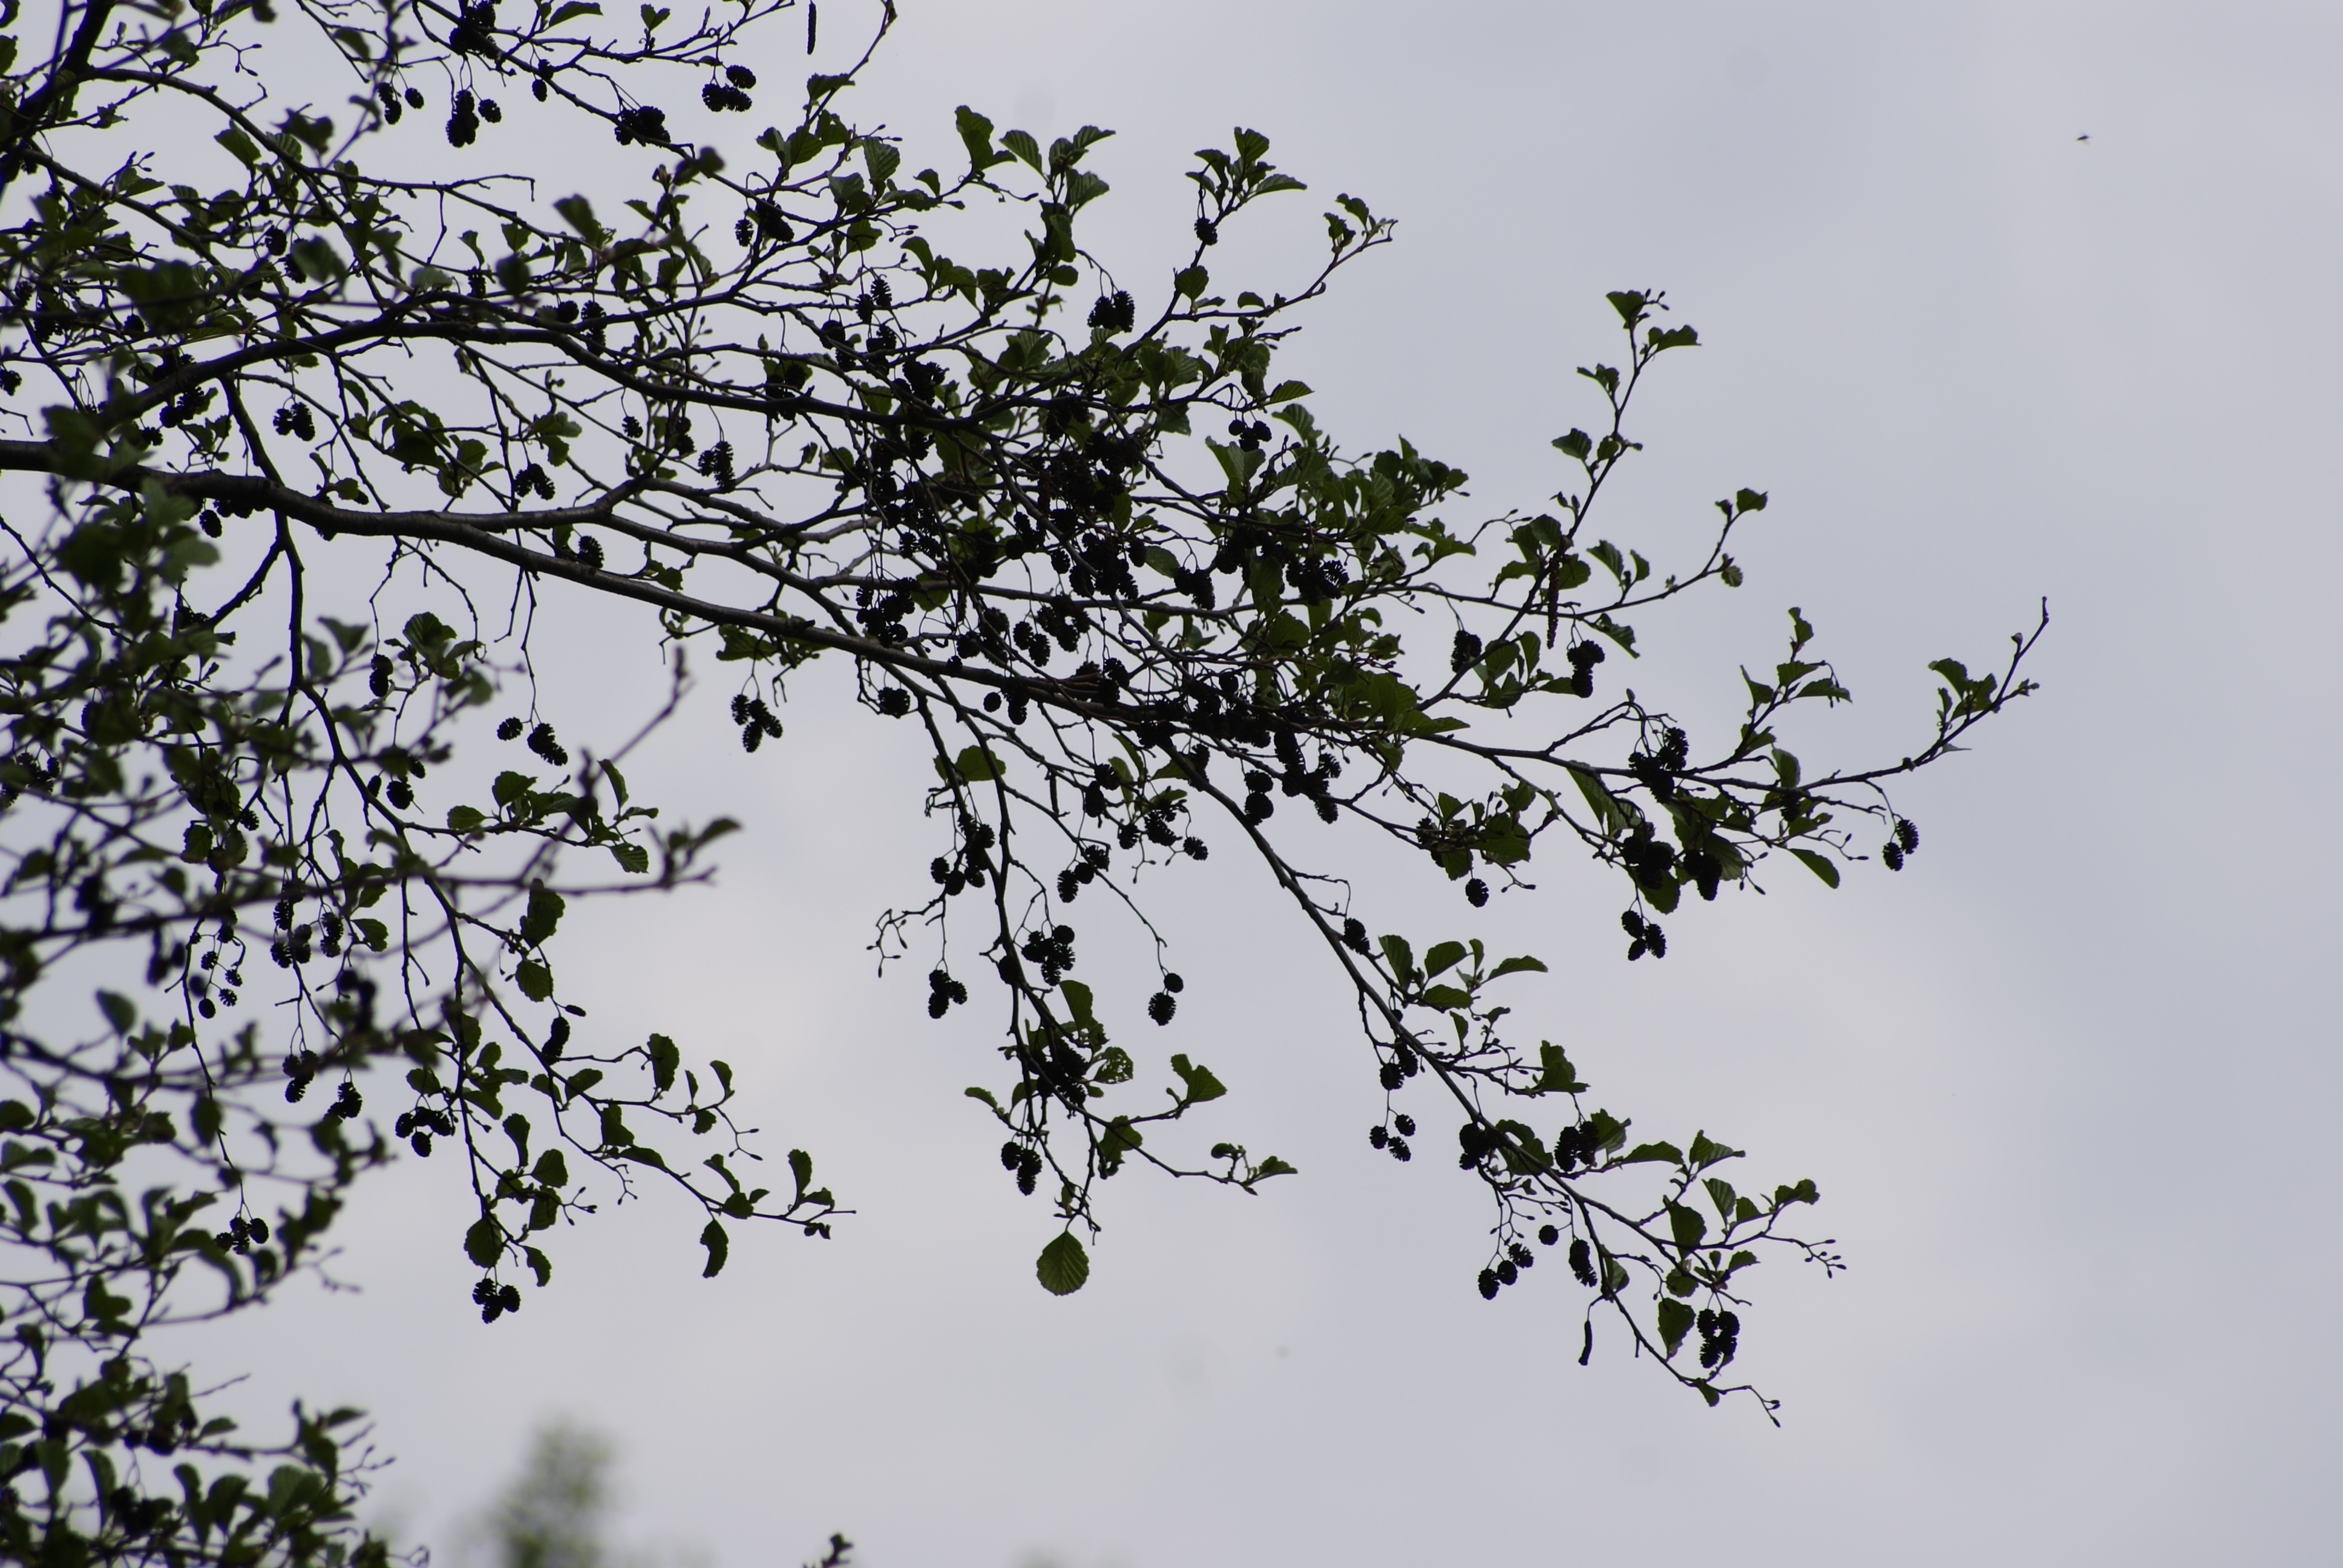
\includegraphics[width=90mm]{obr.jpg}
\caption{podpisisi}
\end{figure}
\chapter{Rozwiązanie - prezentacja wyników}


Zrealizowana aplikacja składa się z dwóch części, tj. aplikacji na adroida oraz
serwera www. Serwer, czyli Servlet(aplet Javy) posiada połączenie z bazą
danych, w której przechowywane są informacje o przesyłce, kurierach i
klientach. 

Aplikację zrealizowano w środowisku programistycnym Eclipse.

schemat - wejscie (adnroid) - środek system - wyjscie www z mapka

\emph{\color{komentarz} dopisac pierdół wstępowych\\oprócz tego dopisać jak
testowałam to}
\section{Aplikacja na system Android}


Założeniem aplikacji mobilnej było lokalizowanie kuriera i wysyłanie jego
pozycji na serwer, który zapisuje ją w bazie danych.
Zasada działania aplikacji polega na odpytaniu kuriera o jego numer id, a
następnie sprawdzeniu czy jest włączony GPS. Ponadto aplikacja wykrywa czy
wprowadzono poprawne id oraz zapobiega zalogowaniu się dwóch kurierów na tym
samym id. Po wpisaniu poprawnego id kuriera aplikacja zapamiętuje go i do
automatycznie wysyła swoją pozycję.

\begin{wrapfigure}{r}{0.5\textwidth}
\centering
\captionsetup{justification=centering,margin=1cm}
\vspace{-20pt}
\begin{center}
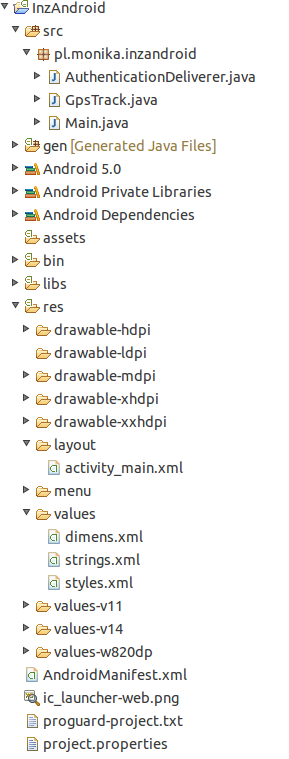
\includegraphics[width=0.2\textwidth]{struktura_android.png}
\end{center}
\vspace{-20pt}
  \caption{Struktura programu aplikacji Android}
\vspace{-10pt}
\label{android}
\end{wrapfigure}

Stworzenie aplikacji na system Android zostało rozpoczęte od doinstalowania
pluginu ADT (Android Development Kit) do programu Eclipse. Na ADT składają się
elementy Android SDK, gdzie SDK to Software Development Kit. Android SDK
zawiera w sobie takie elementy jak Tools - służy do tworzenia aplikacji niezależnie od
wersji systemu Android oraz Platform Tools - narzędzia stworzone pod kątem
wersji systemu Android. W skłąd SDK Tools wchodzą taki funkcjie jak zarządznie
projaektami, modułami czy maszynami wirualnymi, debugger, emulator. Natomiast
Platform Tools zawiera biblioteki do systemu Android. Plugin ADT  korzysta
z funckji Android SDK i pomaga tworzyć, budować, instalować oraz debugować
aplikacje na system Android w środowisku Eclipse. W programie Eclipse tworzona
jest z aplikacją odpowiednia struktura projektu [rys. \ref{android}], w której
jest podział na klasy zawierające logikę aplikacji (scr), pliki generowane przez kompilator (gen),
folder na pliki z zasobami (assets), pliki binarne(bin), dodatkowe biblioteki
(libs) oraz folder na zasoby(res), którego odróżnia od assets to, że są
generowane do pliku R.java (nie trzeba podawać lokalizacji zasobów tylko jego
nazwę). W katalogu res również ustalana jest konfiguracja systemu - 
,,AndroidManifest.xml'', layout (wygląd i ustawienie elementów na ekranie
systemu Android), w podfolderach drawable pliki graficzne, w podfolderach values
ciągi znaków(stringi, kolory) i ustawienia oraz w katalogu menu, w którym
ustawiane są dostępne opcje menu.

Projektowanie aplikacji Android zaczyna się od ustawienia layoutu aplikacji
(/res/layout/activity\_main.xml). Zaprojektowany przez autora layout jest
prosty i przejrzysty, ponieważ ma wykonywać bardzo podstawowe funkcjie. I tak
zawiera w sobie pole do wpisywania id kuriera, pole wyświetlające komunikaty
oraz przycisk wyłączający aplikację. Aplikacja została tak przemyślana, że
aby ją wyłączyć trzeba użyć przycisku ,,Off'', pozostałe hardwar'owe przyciski
nie wyłączają aplikacji, jedynie ją mimalizują. Takie właściwości zostały
stworzone z myślą o tym, aby kurier podczas używania aplikacji tylko w świadomy
sposób mógł ją zamknąć.






 Nie tylko gps do lokalizacji, bo także odbicia
na czytnikach u kurierów Projekt opiera się 



Tu udaje kod
\lstset{style=listJava}
\begin{lstlisting}[caption={to jest podpis}]
class Srass {
	public kupaGowna() {
	} //takakaka
}
\end{lstlisting}
\lstset{style=listPython}
\begin{lstlisting}[caption={to jest podpis drugiego}]
class Srass {
	public kupaGowna() {
	} //takakaka
}
\end{lstlisting}

Udałam kod
\chapter{Przygotowanie i uruchomienie aplikacji}

Że trzeba stworzyć androida, i servlet i bazę danych

\chapter{Wykorzystane technologie}

Zrealizowany tu projekt bazuje na nowoczesnych technologiach.
Skorzystano z mobilnego urządzenia - telefonu komórkowego z systemem
Android, bazy danych do przechowywania inforamcji, a także serweru, który to
łączy wszystkie elementy w jedną spójną całość. Głównym językiem
programowania wykorzystanym w projekcie jest język Java, dzięki któremu
zrelizowano aplikację mobilną, obsługę servletu, bazy danych, odpytywania i
parsowania odpowiedzi serwera Google o widok mapy i odległośći pomiędzy dwoma
punktami, a także obsługa witryny http. Całą oplikację stworzono za pomocą IDE
Eclipse z odpowiednimi dodatkami.
\emph{\color{komentarz}logo Javy}

\section{Java}

Java jest obiektowym językiem programowania ogólnego przeznaczenia.
Charakteryzuje się silnym ukierunkowaniem na obiektowość oraz niezależnością i
przenoszalnośćią kodu od architekty.Oprócz wyżej wymieniowych założeniami języka
Java jest prostota, sieciowość, niezawodność, bezpieczność, interpretowalność, wysokowydajny,
wielowątkowy, dynamiczny oraz niezależny od architektury. 
\begin{itemize}
  \item Prosty - założeniami autorów języka Java było aby programista bez
  specjalnych szkoleń mógł od razu zacząć pisać w języku Java. Skłądnia została
  oczyszczona (w stostunku do C++) o arytmetykę wskaźnikową, struktury, unie,
  przeciążanie operatorów itd.
  \item Zorientowany obiektowo
  \item Sieciowy - Java poasiada bbiliotekę, która w przystępny sposób umożlwia
  pracę z protokałami http, TCP/IP, ftp
  \item Niezawodny - szczególnie skupiono się na wykrywaniu ewentualnych
  problemów, zapobieganiu sytuacjom, w których może błąd nastąpić oraz
  sprawdzaniu błedów podczas działania programu
  \item Bezpieczny - Java może służyć do zastosowań sieciowych, z tego powodu
  zadbano o możwlie najlepsze zabezpieczenie przed wirusami i ingerexją osób
  trzecich.
  \item Niezależny od architektury - Java kompilowana jest do kodu pośredniego
  (bajtoweg), który następnie jest interpretowany na maszynie wirutalnej Javy,
  która jest dostosowana do odpowiedniego systemu. Maszyna wirtualna Javy(JVM)
  jest zdolna wykonywać program z kodu pośredniego. Z tego powodu jeżyk Java
  stosowany jest na wielu urządzeniach oraz różnych systemach operacyjnych.
  Niestyty konsekwencją przenoszalności kodu jest jego wolniejsze wykonanie.
  \item Przenośny - Java posiada ściśle określone rozmiary typów danych i nie ma
  możliwości zmiany rozmiaru przez proramiste przez co nie następuje np. zmiana
  kolejności bajtów
  \item Interpretowany - \ldots
  \item Wysokowydajny - istnieje możliwość tłumaczenia kodu bajtowego w locie,
  co zwiększa szybkość ładowania się programu
  \item Wielowątkowy - pozwala na interaktywność między procesami, a także pracę
  w czasie rzeczywistym
  \item Dynamiczny - obiekty w Javie można zmieniać w zależności od
  zmieniającego się środowiska oraz możliwy jest wgląd we wszystkie obiekty, a
  nawet dodawać nowe metody
\end{itemize}

Język Java wywodzi się z języków C++ i C, wykorzystuje wiele potrzebnych i
użytecznych funkcjonalności tych języków, z nieużytecznych, trudnych lub
pwoowdujących często błędy zrezygnowano. Język Java umożliwia dziedziczenie, a
ponadto wszystkie obiekty Javy są pochodną obiektu bazwego. Jednakże Java nie
umożliwa dziedziczenia wielobazowego, dlatego do Javy wprowadzono interfejsy -
abstrakcyjny typ, który posiada jedynie opracje, ale nie posiada danych, z tego
powodu można tylko implementować interfejs i nie można utworzyć obiektów tego
typu. Język Java umożliwia pisanie aplikacji stacjonarnych, webowych czy
mobilnych. Język Java ma rozbudowaną obsługę wyjątków. Posiada dobrze
rozbudowanego GarbageCollector (odśmieciacza) \cite{java.doc}.
\subsection{podpodrozdział}

\section{Wzorzec architektoniczny - MVC}

W projekcie do zorganizowania struktury aplikacji serwerowej został zastosowany
wzorzec architektoniczny MVC (Model-View-Controller). W modelu tym Model jest
odpowiedzialny za przehcowywanie logiki, z której korzystają inne składowe
systemu. Kolejną częścią składową tej struktury jest Widok, który to jest
odpowiedzialny za funkcje prezentacji w ramach interfejsu użytkownika, ale
także może posiadać swoją logikę. Ostatnim elementem systemu jest Kontroler,
który spaja dwie wcześniejsze cześći. Kontroler odpowiada za przepływ danych
od/do użytkownika, reakcję systemu w zależności od zachowania użytkownika,
kontroler także zarządza Modelem i Widokiem. Takiej strukturze jest jasno
zdefiniowane, która część systemu pełni jakie funkcjie. Taka struktura
architektoniczna jest najczęściej stosowana w aplikacjiach www, gdzie widać
wyraźną grnicę pomiędzy widokiem i modelem, a kontrolerem jest serwer, który
obsługuje informacje płynące z widoku (z http), odpowiednio formuje model i
przekazuje go do widoku. \cite{java.mvc}

\begin{figure}[ht!]
\centering
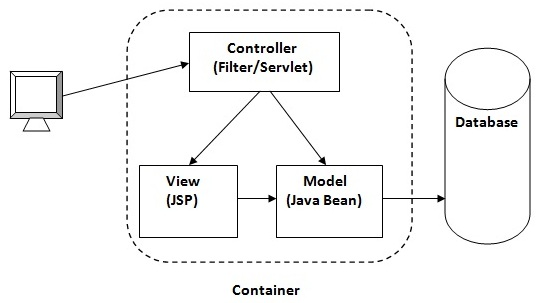
\includegraphics[width=90mm]{model2.jpg}
\caption{Schemat systemu Model-View-Controller model 2\cite{java.mvc.grafika}}
\label{MVC2}
\end{figure}

Autor w swojej pracy użył modelu MVC2 [rys. \ref{MVC2}]
Uzasadnieniem użycia tego wzorca jest ułatwiona organizacja aplikacji, w której
istnieje interfejs graficzny użytkownika. Dzięki niemu w prosty logiczny sposób
można było rozdzielić logikę, kontrolę i widok. Kontenerem z [rys. \ref{MVC2}]
jest opisany w kolejnym podrozdziale Servlet.

\section{Servlet}

Serwlety są to aplikacje działające na serwerze WWW korzystające z języka Java.
Serwlety mają zapewniać budowanie aplikacji internetowych niezależnych od
platformy. Serwlet umożliwia korzystanie z baz danych i http. Z tego powodu
wykrozystywane są do budowania interaktywnych aplikacji internetowych. 
\begin{wrapfigure}{r}{0.5\textwidth}
\label{apache}
\centering
\captionsetup{justification=centering,margin=1cm}
\vspace{-20pt}
\begin{center}
\subfigure {
	
\includegraphics[width=8ex\textwidth]{feather.png}
}
\subfigure{
	
\includegraphics[width=8ex\textwidth]{tomcat.png}
}
\end{center}
\vspace{-20pt}
\caption{Logo Apache i Apache Tomcat \cite{apache.org}}
\vspace{-10pt}
\end{wrapfigure}

open source'owy i korzysta z licencji Apache. Serwer Apache obsługuje www za pomocą protokołu
W projekcie skorzystano z serwletu Tomcat Apache [rys. \ref{apache}], który jest
http, jest otwarty, zapewnia wielowątkowość, skalowalność, bezpieczeństwo,
kontrolę dostępu \cite{apache.wiki}. 


Wybór Tomcate Apache na serwer podyktowany był przez wybór jako głównego języka
aplikacji - Javy. Serwlet jest dość popularnym narzędziem, co pomogło także w
uruchomieniu i skonfigurowaniu go.
\section{JSP - Java}
\section{Technologie internetowe}

W przedstawionym w tej pracy projekcie korzystano z technologi internetowych,
które obsługiwały interakcję z użytkownikiem oraz `strony www`. Skorzystano
z takich technologii jak:
\begin{itemize}
  \item JavaScript - jest to skryptowy jezyk programowania stosowany do
  tworzenia stron internetowych, zapewnia interakcję z użytkownikiem\cite{javascript.wiki}
  \item XML - jesto to język znaczników przeznaczony do reprezenowania danych w
  strukturyzowany sposób \cite{xml.wiki}
  \item Protokół http - 
  \item \ldots
\end{itemize}
\section{db - MySQL}

W projekcie do przechowywania danych skorzystano z baz danych. Baza danych
pozwala w ustrukturyzowany sposób kolekcjonować dane niezbędnę do działania
programów. Przechowywane dane mogą być o dowolnonym formacie i strukturze.

Systemem, do zarządzania bazą danych w projekcie był MySQL. Jest opensource'owe
rozwiązanie do zarządzania relacyjnymi bazami danych. Charakteryzuje się takimi
cechami jak szybki, wielowątkowy dostęp z możliwośćią obsłużenia dużej ilości
użytkowników. Serwer MySQL może być stosowany do systemów, w których znajdują
się dane o znaczeniu krytycznym lub te systemy są mocno obciążane. \cite{Mysql.com} 

\section{Android}

Android jest systemem wykorzystywanym na platformach mobilnych. Android
jest systemem operacyjnym z rodziny Linux, oparty na jądrze Linux. Android
umożliwia tworzenie aplikacji na wiele urządzeń, optymalizacji podlega plik xml,
gdzie można dostosować aplikację do konkretnych urządzeń. Najnowższą wersją
systemu jest Android Lollipop 5.0. 

Rozpoczęcie pracy z Androidem zaczyna się od instalacji środowiska, może to być
Eclipse z dodatkiem SDK Android lub Android Studio. A samo tworzenie aplikacji
od projektu interfejsu użytkownika, następnie dopiero oprogramowuje się obsługę
oraz logikę aplikacji, ostatnim etapem jest testowanie aplikacji.
\cite{developer.android}
\emph{\color{komentarz}napisac o tym, ze android oddelegowuje zadania, taki
obrazek ze strony}

\section{Google apps - mapy}

Firma Google udostępnia korzystanie deweloperom ze swoich produktów
\cite{developer.google}. W swoim projekcie korzystałam z Google Maps Api. 

\chapter{Możliwość rozwinięcia w przyszłości}
Aplikację można „podpiąć” pod prawdziwe urządzenia jakie posiadają kurierzy – te na których się człowiek podpisuje – ale konieczne będzie 
zrefakturyzowanie(?)/zmienie kodu pod system, który mają tam zainstalowany.
	Fajnie by było to wrzycić na prawdziwe tablety, można by sprzedawać/zarobić. Ogólnie koszt takiego urządzenia to byłoby tablet/telefon 
	+ wycena za program.
	Normalnie kurierzy urzywają kolektorów danych.

\chapter{Wnioski i podsumowanie}
\addcontentsline{toc}{chapter}{Bibliografia} %utworzenie w spisie tresci pozycji Bibliografia
\bibliography{bibliografia} % wstawia bibliografie korzystajac z
% pliku bibliografia.bib - dotyczy BibTeXa, jezeli nie korzystamy z BibTeXa nalezy uzyc otoczenia thebibliography

%opcjonalnie moze sie tu pojawic spis rysunkow i tabel
\listoffigures
\listoftables
\lstlistoflistings
\end{document}
